\documentclass{beamer}
 
\usepackage[utf8]{inputenc}
\def\Put(#1,#2)#3{\leavevmode\makebox(0,0){\put(#1,#2){#3}}}
\usepackage{tikz}
  
   
%Information to be included in the title page:
\title{Solar-Electric and Gas Powered, Long-Endurance UAV Sizing via Geometric Programming}
\author{Michael Burton and Warren Hoburg}
\institute{Massachusetts Institute of Technology}
\date{Feb 14, 2017}
 
\begin{document}
 
\frame{\titlepage}
 
\begin{frame}

\frametitle{Long-endurance UAV Applications}
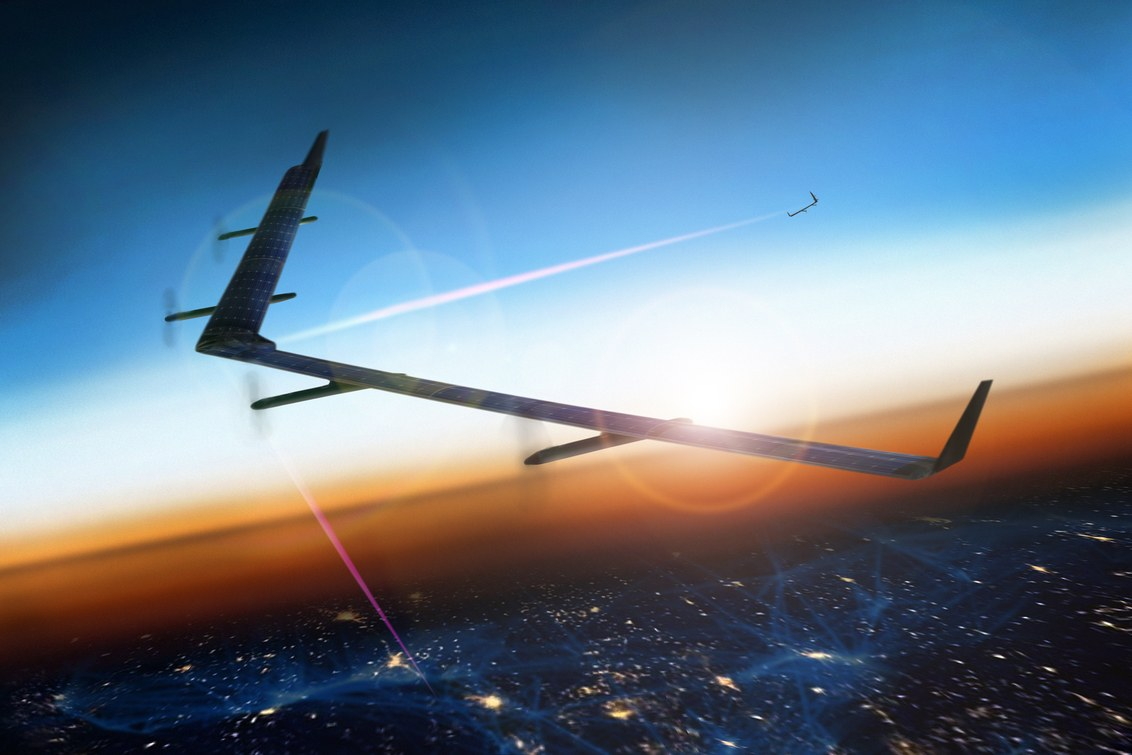
\includegraphics[height=4cm]{aquila.jpg}
    \pause
\Put(-130,90){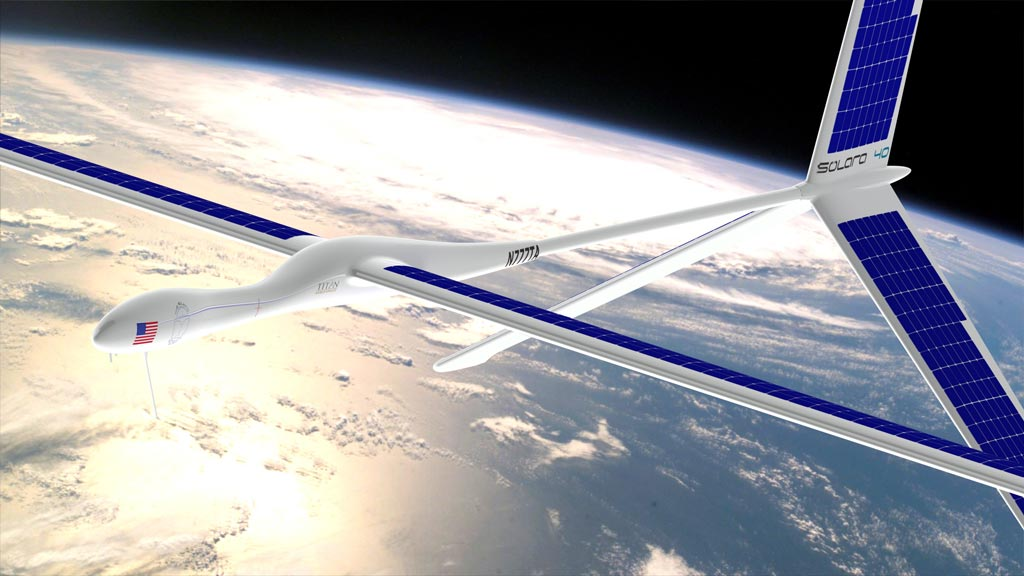
\includegraphics[height=4cm]{titan.jpg}}
    \pause
\Put(-110,80){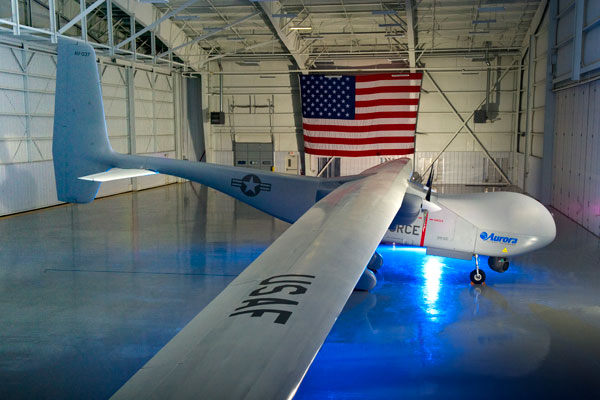
\includegraphics[height=4cm]{orion.jpg}}
    \pause
\Put(-90,70){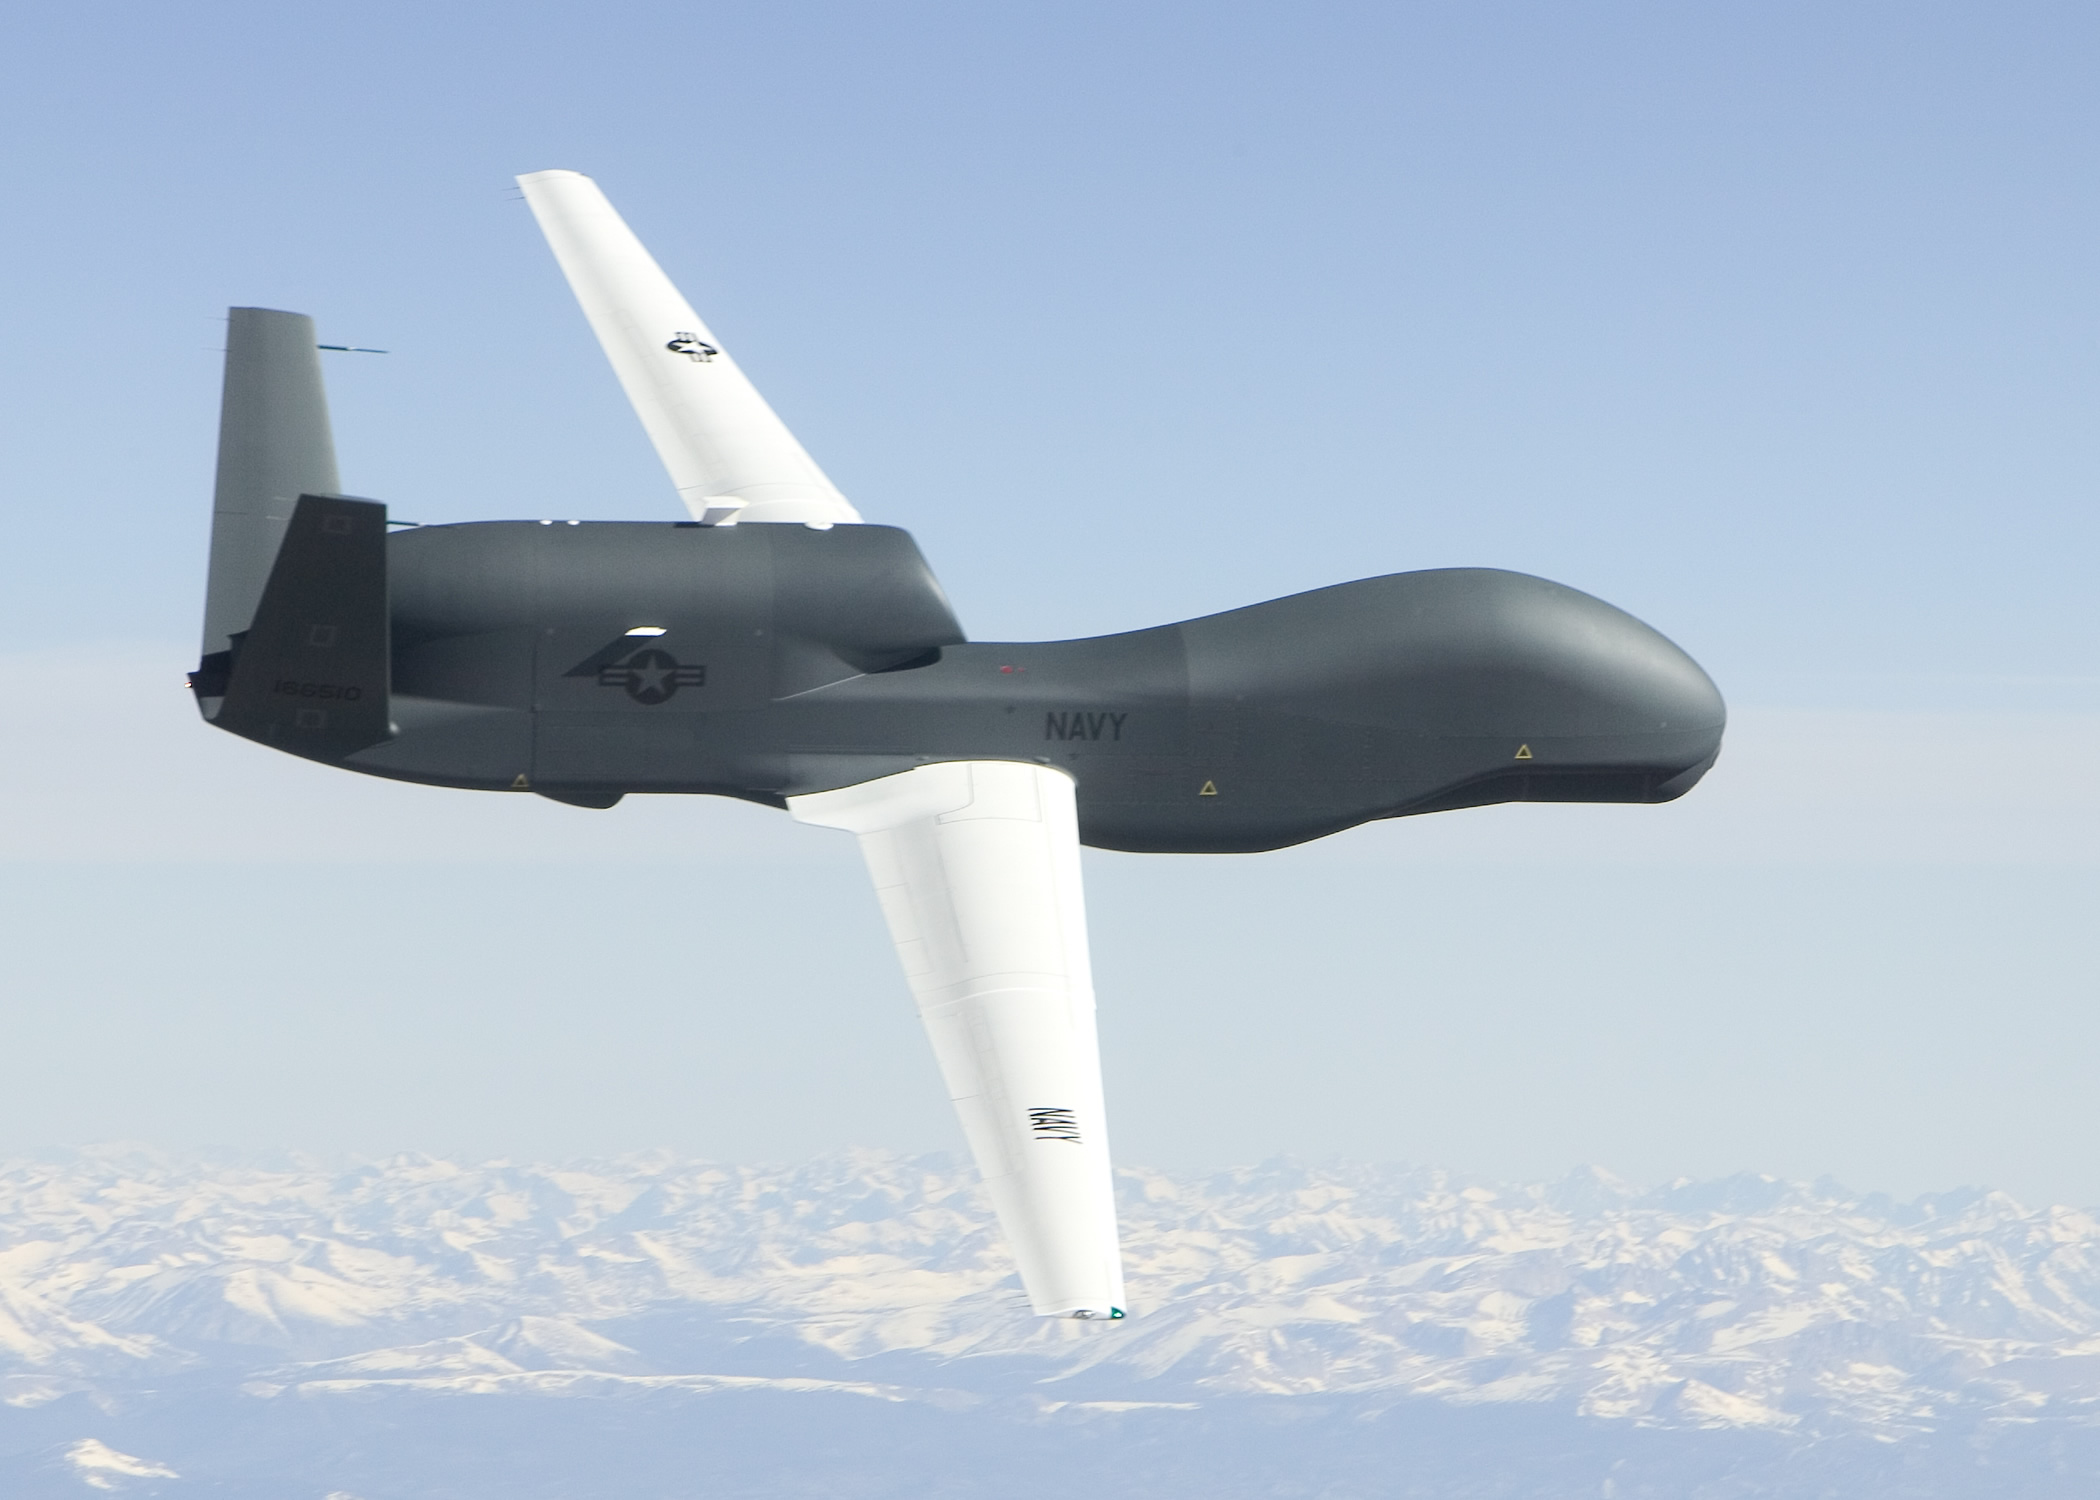
\includegraphics[height=4cm]{globalhawk.jpg}}
    \pause
\Put(-70,60){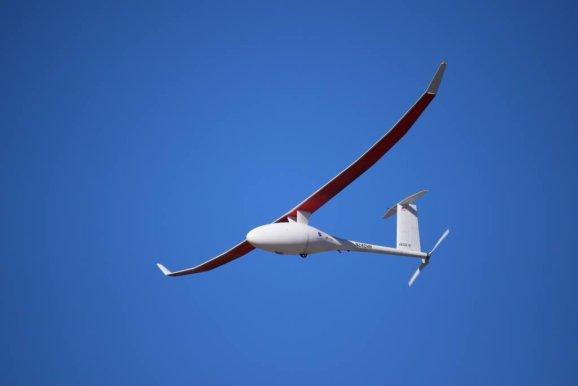
\includegraphics[height=4cm]{vanilla.jpg}}
    \pause
\Put(-70,60){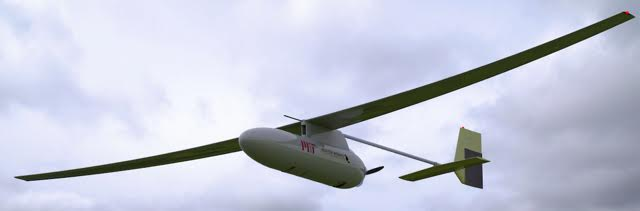
\includegraphics[height=3cm]{jho.jpeg}}

\end{frame}
 
\begin{frame}
    \frametitle{Limitations on Endurance}

    \begin{itemize}
        \item Gas: fuel 
        \item Solar-electric: winter solstice \\~\\
    \end{itemize}

    
    At 30$^{\circ}$ latitude:
    \begin{columns}
        \column{0.5\textwidth}
        \includegraphics[width=1.0\textwidth]{windvsmonth.pdf}
        
        \column{0.5\textwidth}
        \includegraphics[width=1.0\textwidth]{eirrvsmonth.pdf}
    \end{columns}

\end{frame}

\begin{frame}
    \frametitle{Operational Capability}

    Latitude requirement = cability to operate within band of latitudes

    \includegraphics[width=0.5\textwidth]{latvswind.pdf}

\end{frame}

\begin{frame}
    \frametitle{Operating Altitude}
    
    \begin{columns}
        \column{0.4\textwidth}
        \begin{itemize}
            \item Gas: determine by payload
                \begin{itemize}
                    \item (5,000 - 25,000 ft)
                    \end{itemize}
            \item Solar-electric: optimized 
                \begin{itemize}
                    \item (55,000 - 70,000 ft)
                    \end{itemize}
                \end{itemize}
        
        \column{0.6\textwidth}
        \includegraphics[width=1.0\textwidth]{altvswind.pdf}
    \end{columns}

\end{frame}

\begin{frame}
    \frametitle{Percentile Wind Speed}
    
    \begin{columns}
        \column{0.5\textwidth}
        \includegraphics[width=1.0\textwidth]{Boston_dec_2015.pdf}
        
        \column{0.5\textwidth}
        \includegraphics[width=1.0\textwidth]{Boston_dec_2015auto.pdf}
    \end{columns}
    
\end{frame}

\begin{frame}
    \frametitle{Geometric Programming}
    \begin{itemize}
        \item Non-linear optimization
        \item Can be solved extremely quickly
        \item Guaranteed global optimum
        \item No initial guess
        \end{itemize}
\end{frame}

\begin{frame}
    \frametitle{Example GP}

    \begin{columns}
        \column{0.5\textwidth}
        Form:
        \column{0.5\textwidth}
        Example:
    \end{columns}
    
    \begin{columns}
        \column{0.5\textwidth}
        \scriptsize
        \begin{align*}
            \text{minimize } &g_0(x) \\
            \text{subject to } &f_i(x) = 1, &i &= 1,\dots,m\\
                               &g_i(x) \leq 1, &i &= 1,\dots,n
        \end{align*}

        \begin{align*}
            f(\bold{x}) &= c x_1^{a_1} x_2^{a_2} \dotsm x_n^{a_n} , \\
            g(\bold{x}) &= \displaystyle\sum_{k=1}^K c_k x_1^{a_{1_k}} x_2^{a_{2_k}} \dotsm x_n^{a_{n_k}}.
        \end{align*}

        \column{0.5\textwidth}
        \scriptsize
        \begin{align*}
            \text{minimize } & x^{-1}y^{-1/2}z^{-1} + 2.3xz + 4xyz\\
            \text{subject to } &\frac{1}{3}x^{-2}y^{-2} + \frac{4}{3}y^{1/2}z^{-1} \leq 1\\
                              &x + 2y + 3z \leq 1
        \normalsize
        \end{align*}

    \end{columns}
\end{frame}

\begin{frame}
    \frametitle{Optimizing Wind Speed}

    \begin{align*}
        V &\geq V_{\text{wind}_i}, i = 20,\dots,n \\
        V_{\text{wind}} &= f(\rho, p_{\text{wind}})
    \end{align*}

    Latitude requirement = $n$ \\~\\

    \begin{center}
    \includegraphics[width=0.6\textwidth]{windfitl35.pdf}
    \end{center}

\end{frame}

\begin{frame}
    \frametitle{Solar Energy}

    \scriptsize
    \[ \begin{array}{lcl}
        \text{Solar Energy} : & (E/S)_{\text{sun}}  &\geq (E/S)_{\text{day}} + \frac{E_{\text{batt}}}{\eta_{\text{charge}}\eta_{\text{solar}} S_{\text{solar}}} \\
        \text{Battery Energy} : &E_{\text{batt}} &\geq \frac{P_{\text{oper}}t_{\text{night}}}{\eta_{\text{discharge}}} + (E/S)_{\text{twilight}} \eta_{\text{solar}} S_{\text{solar}} \\
        \text{Minimum operational solar power} : & (P/S)_{\text{min}} &= \frac{P_{\text{oper}}}{\eta_{\text{solar}} S_{\text{solar}}} 
    \end{array} \]

    \begin{center}
    \includegraphics[width=0.6\textwidth]{lat30.pdf}
    \end{center}
\end{frame}

\end{document}
